\documentclass[11pt]{article}
% Manuscript for npj Computational Materials (Article).
% Numbers marked \pd{...} come from pd_numbers.tex (make_report_numbers.py), fr_numbers.tex
% (make_final_numbers.py) and ms_numbers.tex (make_manuscript_tables.py). Build the
% supplementary file first, so that its table and figure numbers can be cited here:
%   latexmk -pdf -outdir=build npj_supplementary.tex npj_manuscript.tex
\usepackage[letterpaper,margin=1in]{geometry}
\usepackage[T1]{fontenc}
\usepackage[utf8]{inputenc}
\usepackage{mathptmx}
\usepackage{amsmath,amssymb,bm}
\usepackage{microtype}
\usepackage{booktabs}
\usepackage{graphicx}
\usepackage{xcolor}
\usepackage{tabularx}
\usepackage[numbers,super,sort&compress]{natbib}
\usepackage[labelfont=bf,labelsep=period,font=small]{caption}
\usepackage{setspace}
\usepackage[mathlines]{lineno}
\usepackage{xr}
\externaldocument[S-]{build/npj_supplementary}
\usepackage[colorlinks=true,linkcolor=black,citecolor=black,urlcolor=blue!50!black]{hyperref}
\hypersetup{pdftitle={Finding point defects in a model glass from atomic positions with neural networks},pdfauthor={Stacy Cheruto, Nicholaus Ladislaus, Abubakar Chilala, Gentille Uwera, Michel Sangwa, Boniface Godwin}}
\renewcommand{\figurename}{Fig.}
\setlength{\parskip}{4pt}
\makeatletter
\newcommand{\pd}[1]{\@ifundefined{pd@#1}{\textcolor{red}{[#1]}}{\csname pd@#1\endcsname}}
\newcommand{\pdset}[2]{\expandafter\gdef\csname pd@#1\endcsname{#2}}
\makeatother
\IfFileExists{pd_numbers.tex}{% written by make_report_numbers.py
\pdset{abl-diff-layers1}{6.2}
\pdset{abl-diff-layers2}{1.3}
\pdset{abl-diff-no-weights}{1.2}
\pdset{abl-diff-real-only}{0.0}
\pdset{abl-diff-scratch}{22.0}
\pdset{abl-label-layers1-interstitial}{0}
\pdset{abl-label-layers1-vacancy}{0}
\pdset{abl-label-layers2-interstitial}{0}
\pdset{abl-label-layers2-vacancy}{0}
\pdset{abl-label-no-weights-interstitial}{0}
\pdset{abl-label-no-weights-vacancy}{7}
\pdset{abl-label-real-only-interstitial}{17}
\pdset{abl-label-real-only-vacancy}{32}
\pdset{abl-label-reference-interstitial}{18}
\pdset{abl-label-reference-vacancy}{27}
\pdset{abl-label-scratch-interstitial}{0}
\pdset{abl-label-scratch-vacancy}{0}
\pdset{abl-layers1-all}{15.6}
\pdset{abl-layers1-antisite}{14.2}
\pdset{abl-layers1-frenkel}{13.8}
\pdset{abl-layers1-high}{17.3}
\pdset{abl-layers1-interstitial}{21.8}
\pdset{abl-layers1-low}{14.8}
\pdset{abl-layers1-sd}{1.5}
\pdset{abl-layers1-vacancy}{12.3}
\pdset{abl-layers2-all}{20.6}
\pdset{abl-layers2-antisite}{20.8}
\pdset{abl-layers2-frenkel}{21.3}
\pdset{abl-layers2-high}{23.1}
\pdset{abl-layers2-interstitial}{26.5}
\pdset{abl-layers2-low}{18.3}
\pdset{abl-layers2-sd}{2.4}
\pdset{abl-layers2-vacancy}{13.8}
\pdset{abl-lower-layers1}{3}
\pdset{abl-lower-layers2}{3}
\pdset{abl-lower-no-weights}{3}
\pdset{abl-lower-real-only}{2}
\pdset{abl-lower-scratch}{3}
\pdset{abl-no-weights-all}{42.7}
\pdset{abl-no-weights-antisite}{39.5}
\pdset{abl-no-weights-frenkel}{35.1}
\pdset{abl-no-weights-high}{43.5}
\pdset{abl-no-weights-interstitial}{31.0}
\pdset{abl-no-weights-low}{41.6}
\pdset{abl-no-weights-sd}{1.0}
\pdset{abl-no-weights-vacancy}{63.2}
\pdset{abl-real-only-ahead}{2.5}
\pdset{abl-real-only-all}{43.8}
\pdset{abl-real-only-antisite}{40.2}
\pdset{abl-real-only-behind}{2.5}
\pdset{abl-real-only-frenkel}{38.0}
\pdset{abl-real-only-high}{46.1}
\pdset{abl-real-only-interstitial}{30.8}
\pdset{abl-real-only-low}{42.1}
\pdset{abl-real-only-sd}{2.1}
\pdset{abl-real-only-vacancy}{64.7}
\pdset{abl-reference-all}{43.8}
\pdset{abl-reference-antisite}{41.7}
\pdset{abl-reference-frenkel}{38.7}
\pdset{abl-reference-high}{44.7}
\pdset{abl-reference-interstitial}{30.7}
\pdset{abl-reference-low}{43.2}
\pdset{abl-reference-sd}{0.8}
\pdset{abl-reference-vacancy}{63.0}
\pdset{abl-scratch-all}{21.9}
\pdset{abl-scratch-antisite}{24.2}
\pdset{abl-scratch-frenkel}{22.2}
\pdset{abl-scratch-high}{23.7}
\pdset{abl-scratch-interstitial}{26.8}
\pdset{abl-scratch-low}{18.7}
\pdset{abl-scratch-sd}{2.8}
\pdset{abl-scratch-vacancy}{14.3}
\pdset{abl-seeds}{three}
\pdset{abl-updates}{2,000}
\pdset{chance-antisite}{4}
\pdset{chance-frenkel}{5.4}
\pdset{chance-interstitial}{3}
\pdset{chance-max}{5}
\pdset{chance-min}{3}
\pdset{chance-vacancy}{2.9}
\pdset{exp-20k}{50.3}
\pdset{exp-60k}{54}
\pdset{exp-p-cal}{$p<0.001$}
\pdset{exp-p-length}{$p=0.001$}
\pdset{exp-uncal}{50.7}
\pdset{fin-by-all}{36--37}
\pdset{fin-by-none}{36--38}
\pdset{fin-by-one}{62--64}
\pdset{fin-cnn-all}{54.0}
\pdset{fin-cnn-antisite}{52.8}
\pdset{fin-cnn-frenkel}{38.4}
\pdset{fin-cnn-high}{54.4}
\pdset{fin-cnn-hours}{0.6}
\pdset{fin-cnn-interstitial}{51.2}
\pdset{fin-cnn-low}{53.5}
\pdset{fin-cnn-noshift}{12}
\pdset{fin-cnn-shift}{88}
\pdset{fin-cnn-size}{0.50}
\pdset{fin-cnn-vacancy}{69.7}
\pdset{fin-cnn3-all}{54.7}
\pdset{fin-cnn3-antisite}{54.0}
\pdset{fin-cnn3-frenkel}{38.7}
\pdset{fin-cnn3-hi}{59}
\pdset{fin-cnn3-interstitial}{51.5}
\pdset{fin-cnn3-lo}{51}
\pdset{fin-cnn3-p}{$p=0.86$}
\pdset{fin-cnn3-vacancy}{70.5}
\pdset{fin-egnn-all}{43.5}
\pdset{fin-egnn-antisite}{44.0}
\pdset{fin-egnn-frenkel}{35.1}
\pdset{fin-egnn-high}{43.9}
\pdset{fin-egnn-hours}{0.8}
\pdset{fin-egnn-interstitial}{29.7}
\pdset{fin-egnn-low}{42.9}
\pdset{fin-egnn-noshift}{0}
\pdset{fin-egnn-shift}{100}
\pdset{fin-egnn-size}{0.52}
\pdset{fin-egnn-vacancy}{63.2}
\pdset{fin-egnn3-all}{44.0}
\pdset{fin-egnn3-antisite}{45.5}
\pdset{fin-egnn3-frenkel}{32.7}
\pdset{fin-egnn3-hi}{48}
\pdset{fin-egnn3-interstitial}{30.0}
\pdset{fin-egnn3-lo}{40}
\pdset{fin-egnn3-p}{$p=1.00$}
\pdset{fin-egnn3-vacancy}{65.0}
\pdset{fin-lost-cnn}{38--42}
\pdset{fin-lost-pre}{43}
\pdset{fin-lost-tr}{34--41}
\pdset{fin-main-all}{54.0}
\pdset{fin-main-antisite}{49.0}
\pdset{fin-main-frenkel}{45.3}
\pdset{fin-main-interstitial}{50.0}
\pdset{fin-main-noshift}{0}
\pdset{fin-main-shift}{100}
\pdset{fin-main-size}{0.52}
\pdset{fin-main-vacancy}{69.5}
\pdset{fin-only-cnn}{114--122}
\pdset{fin-only-pre}{91}
\pdset{fin-only-tr}{110--116}
\pdset{fin-p-cnn}{$p<0.001$}
\pdset{fin-p-pre}{$p<0.001$}
\pdset{fin-p-tr}{$p<0.001$}
\pdset{fin-p-tr-cnn}{$p=0.49$--$0.91$}
\pdset{fin-p-tr-cnn-antisite}{0.33}
\pdset{fin-p-tr-cnn-frenkel}{0.25}
\pdset{fin-p-tr-cnn-interstitial}{0.04}
\pdset{fin-p-tr-cnn-vacancy}{0.12}
\pdset{fin-pair-all}{55.2}
\pdset{fin-pair-antisite}{55.5}
\pdset{fin-pair-frenkel}{41.3}
\pdset{fin-pair-hi}{59}
\pdset{fin-pair-interstitial}{51.5}
\pdset{fin-pair-lo}{51}
\pdset{fin-pair-p}{$p=0.090$}
\pdset{fin-pair-vacancy}{69.0}
\pdset{fin-pre-all}{50.3}
\pdset{fin-pre-antisite}{46.5}
\pdset{fin-pre-frenkel}{36.7}
\pdset{fin-pre-interstitial}{47.5}
\pdset{fin-pre-noshift}{0}
\pdset{fin-pre-shift}{100}
\pdset{fin-pre-size}{0.52}
\pdset{fin-pre-vacancy}{67.0}
\pdset{fin-report-all}{55.2}
\pdset{fin-report-antisite}{55.0}
\pdset{fin-report-frenkel}{41.3}
\pdset{fin-report-hi}{59}
\pdset{fin-report-interstitial}{51.0}
\pdset{fin-report-lo}{51}
\pdset{fin-report-p}{$p=0.30$}
\pdset{fin-report-vacancy}{70.0}
\pdset{fin-six-all}{55.1}
\pdset{fin-six-antisite}{56.0}
\pdset{fin-six-frenkel}{41.3}
\pdset{fin-six-hi}{59}
\pdset{fin-six-interstitial}{49.5}
\pdset{fin-six-lo}{51}
\pdset{fin-six-p}{$p=0.58$}
\pdset{fin-six-vacancy}{70.0}
\pdset{fin-three-all}{54.1}
\pdset{fin-three-antisite}{54.5}
\pdset{fin-three-frenkel}{40.7}
\pdset{fin-three-hi}{58}
\pdset{fin-three-interstitial}{50.0}
\pdset{fin-three-lo}{50}
\pdset{fin-three-p}{$p=0.77$}
\pdset{fin-three-vacancy}{68.0}
\pdset{fin-tr-all}{53.6}
\pdset{fin-tr-antisite}{54.2}
\pdset{fin-tr-frenkel}{42.0}
\pdset{fin-tr-high}{53.9}
\pdset{fin-tr-hours}{0.6}
\pdset{fin-tr-interstitial}{48.3}
\pdset{fin-tr-low}{53.3}
\pdset{fin-tr-noshift}{0}
\pdset{fin-tr-shift}{100}
\pdset{fin-tr-size}{0.58}
\pdset{fin-tr-vacancy}{67.2}
\pdset{fin-tr3-all}{54.5}
\pdset{fin-tr3-antisite}{56.5}
\pdset{fin-tr3-frenkel}{42.7}
\pdset{fin-tr3-hi}{58}
\pdset{fin-tr3-interstitial}{48.0}
\pdset{fin-tr3-lo}{51}
\pdset{fin-tr3-p}{$p=0.44$}
\pdset{fin-tr3-vacancy}{68.0}
\pdset{fother-found-bonds}{26.2}
\pdset{fother-found-bonds-hi}{36}
\pdset{fother-found-bonds-lo}{17}
\pdset{fother-found-energy}{31}
\pdset{fother-found-energy-hi}{41}
\pdset{fother-found-energy-lo}{22}
\pdset{fother-found-finder}{44}
\pdset{fother-found-finder-hi}{55}
\pdset{fother-found-finder-lo}{33}
\pdset{fother-found-geometry}{20.2}
\pdset{fother-found-geometry-hi}{28}
\pdset{fother-found-geometry-lo}{12}
\pdset{fother-n}{84}
\pdset{fother-p-found-energy}{$p=0.071$}
\pdset{fother-p-restored-energy}{$p=0.77$}
\pdset{fother-restored-bonds}{1.2}
\pdset{fother-restored-bonds-hi}{4}
\pdset{fother-restored-bonds-lo}{0}
\pdset{fother-restored-ceiling}{27.4}
\pdset{fother-restored-ceiling-hi}{38}
\pdset{fother-restored-ceiling-lo}{18}
\pdset{fother-restored-energy}{6}
\pdset{fother-restored-energy-hi}{11}
\pdset{fother-restored-energy-lo}{1}
\pdset{fother-restored-finder}{8.3}
\pdset{fother-restored-finder-hi}{14}
\pdset{fother-restored-finder-lo}{3}
\pdset{fother-restored-geometry}{0}
\pdset{fother-restored-geometry-hi}{4}
\pdset{fother-restored-geometry-lo}{0}
\pdset{found-best-antisite}{31.5}
\pdset{found-best-frenkel}{32.7}
\pdset{found-best-interstitial}{28}
\pdset{found-best-vacancy}{47.5}
\pdset{found-bonds-antisite}{31.5}
\pdset{found-bonds-frenkel}{27.3}
\pdset{found-bonds-interstitial}{28}
\pdset{found-bonds-max}{31.5}
\pdset{found-bonds-min}{27.3}
\pdset{found-bonds-vacancy}{29}
\pdset{found-energy-antisite}{29}
\pdset{found-energy-frenkel}{32.7}
\pdset{found-energy-interstitial}{28}
\pdset{found-energy-max}{32.7}
\pdset{found-energy-min}{28}
\pdset{found-energy-vacancy}{29.5}
\pdset{found-finder-antisite}{49}
\pdset{found-finder-frenkel}{45.3}
\pdset{found-finder-interstitial}{50}
\pdset{found-finder-vacancy}{69.5}
\pdset{found-geometry-antisite}{16.5}
\pdset{found-geometry-frenkel}{26.7}
\pdset{found-geometry-interstitial}{15}
\pdset{found-geometry-max}{47.5}
\pdset{found-geometry-min}{15}
\pdset{found-geometry-vacancy}{47.5}
\pdset{fp-n-anti}{35}
\pdset{fp-n-close}{27}
\pdset{fp-n-complex}{19}
\pdset{fp-n-none}{3}
\pdset{fp-n-pair}{66}
\pdset{fp-n-pair-pure}{40}
\pdset{fpair-found-bonds}{28.8}
\pdset{fpair-found-bonds-hi}{40}
\pdset{fpair-found-bonds-lo}{19}
\pdset{fpair-found-energy}{34.8}
\pdset{fpair-found-energy-hi}{47}
\pdset{fpair-found-energy-lo}{24}
\pdset{fpair-found-finder}{47}
\pdset{fpair-found-finder-hi}{59}
\pdset{fpair-found-finder-lo}{35}
\pdset{fpair-found-geometry}{34.8}
\pdset{fpair-found-geometry-hi}{47}
\pdset{fpair-found-geometry-lo}{24}
\pdset{fpair-n}{66}
\pdset{fpair-p-found-energy}{$p=0.15$}
\pdset{fpair-p-restored-energy}{$p=0.18$}
\pdset{fpair-restored-bonds}{1.5}
\pdset{fpair-restored-bonds-hi}{5}
\pdset{fpair-restored-bonds-lo}{0}
\pdset{fpair-restored-ceiling}{60.6}
\pdset{fpair-restored-ceiling-hi}{71}
\pdset{fpair-restored-ceiling-lo}{49}
\pdset{fpair-restored-energy}{9.1}
\pdset{fpair-restored-energy-hi}{17}
\pdset{fpair-restored-energy-lo}{3}
\pdset{fpair-restored-finder}{18.2}
\pdset{fpair-restored-finder-hi}{28}
\pdset{fpair-restored-finder-lo}{10}
\pdset{fpair-restored-geometry}{0}
\pdset{fpair-restored-geometry-hi}{5}
\pdset{fpair-restored-geometry-lo}{0}
\pdset{frenkel-exact-energy}{7}
\pdset{frenkel-exact-finder}{21}
\pdset{gap-finder-energy-max}{40}
\pdset{gap-finder-energy-min}{20}
\pdset{glass-auc}{0.75}
\pdset{glass-clean-cal}{2}
\pdset{glass-clean-raw}{68}
\pdset{glass-def-cal}{28.7}
\pdset{lead-found-antisite}{18}
\pdset{lead-found-frenkel}{13}
\pdset{lead-found-interstitial}{22}
\pdset{lead-found-max}{22}
\pdset{lead-found-min}{18}
\pdset{lead-found-vacancy}{22}
\pdset{lead-restored-antisite}{22}
\pdset{lead-restored-frenkel}{5}
\pdset{lead-restored-interstitial}{16}
\pdset{lead-restored-vacancy}{13}
\pdset{n-antisite}{200}
\pdset{n-frenkel}{150}
\pdset{n-interstitial}{200}
\pdset{n-test}{750}
\pdset{n-tests-family}{12}
\pdset{n-vacancy}{200}
\pdset{occ-anti}{71}
\pdset{occ-anti-pairlike}{22}
\pdset{occ-int}{95.5}
\pdset{occ-undone}{50}
\pdset{occ-undone-n}{50}
\pdset{occ-vac}{93}
\pdset{p-found-bonds-antisite}{<0.001}
\pdset{p-found-bonds-frenkel}{<0.001}
\pdset{p-found-bonds-interstitial}{<0.001}
\pdset{p-found-bonds-vacancy}{<0.001}
\pdset{p-found-energy-antisite}{<0.001}
\pdset{p-found-energy-frenkel}{0.014}
\pdset{p-found-energy-interstitial}{<0.001}
\pdset{p-found-energy-vacancy}{<0.001}
\pdset{p-found-geometry-antisite}{<0.001}
\pdset{p-found-geometry-frenkel}{0.002}
\pdset{p-found-geometry-interstitial}{<0.001}
\pdset{p-found-geometry-vacancy}{<0.001}
\pdset{p-restored-bonds-antisite}{<0.001}
\pdset{p-restored-bonds-frenkel}{<0.001}
\pdset{p-restored-bonds-interstitial}{<0.001}
\pdset{p-restored-bonds-vacancy}{<0.001}
\pdset{p-restored-energy-antisite}{<0.001}
\pdset{p-restored-energy-frenkel}{0.169}
\pdset{p-restored-energy-interstitial}{<0.001}
\pdset{p-restored-energy-vacancy}{<0.001}
\pdset{p-restored-geometry-antisite}{<0.001}
\pdset{p-restored-geometry-frenkel}{<0.001}
\pdset{p-restored-geometry-interstitial}{<0.001}
\pdset{p-restored-geometry-vacancy}{<0.001}
\pdset{p-worst-found}{p<0.001}
\pdset{p-worst-restored}{p<0.001}
\pdset{praw-found-bonds-antisite}{<0.001}
\pdset{praw-found-bonds-frenkel}{<0.001}
\pdset{praw-found-bonds-interstitial}{<0.001}
\pdset{praw-found-bonds-vacancy}{<0.001}
\pdset{praw-found-energy-antisite}{<0.001}
\pdset{praw-found-energy-frenkel}{0.014}
\pdset{praw-found-energy-interstitial}{<0.001}
\pdset{praw-found-energy-vacancy}{<0.001}
\pdset{praw-found-geometry-antisite}{<0.001}
\pdset{praw-found-geometry-frenkel}{<0.001}
\pdset{praw-found-geometry-interstitial}{<0.001}
\pdset{praw-found-geometry-vacancy}{<0.001}
\pdset{praw-restored-bonds-antisite}{<0.001}
\pdset{praw-restored-bonds-frenkel}{<0.001}
\pdset{praw-restored-bonds-interstitial}{<0.001}
\pdset{praw-restored-bonds-vacancy}{<0.001}
\pdset{praw-restored-energy-antisite}{<0.001}
\pdset{praw-restored-energy-frenkel}{0.169}
\pdset{praw-restored-energy-interstitial}{<0.001}
\pdset{praw-restored-energy-vacancy}{<0.001}
\pdset{praw-restored-geometry-antisite}{<0.001}
\pdset{praw-restored-geometry-frenkel}{<0.001}
\pdset{praw-restored-geometry-interstitial}{<0.001}
\pdset{praw-restored-geometry-vacancy}{<0.001}
\pdset{press-antisite}{16}
\pdset{press-antisite-hi}{22}
\pdset{press-antisite-lo}{11}
\pdset{press-antisite-rule}{lowest}
\pdset{press-frenkel}{10.7}
\pdset{press-frenkel-hi}{16}
\pdset{press-frenkel-lo}{6}
\pdset{press-frenkel-rule}{lowest}
\pdset{press-interstitial}{19}
\pdset{press-interstitial-hi}{25}
\pdset{press-interstitial-lo}{14}
\pdset{press-interstitial-rule}{most unusual}
\pdset{press-max}{19}
\pdset{press-min}{8.5}
\pdset{press-p-antisite}{$p<0.001$}
\pdset{press-p-frenkel}{$p<0.001$}
\pdset{press-p-interstitial}{$p<0.001$}
\pdset{press-p-vacancy}{$p<0.001$}
\pdset{press-ref-a}{6.5\pm5.4}
\pdset{press-ref-b}{2.9\pm5.4}
\pdset{press-vacancy}{8.5}
\pdset{press-vacancy-hi}{12}
\pdset{press-vacancy-lo}{5}
\pdset{press-vacancy-rule}{lowest}
\pdset{press-val-highest}{21}
\pdset{press-val-unusual}{21.5}
\pdset{presscell-antisite}{15}
\pdset{presscell-antisite-hi}{20}
\pdset{presscell-antisite-lo}{10}
\pdset{presscell-antisite-rule}{lowest}
\pdset{presscell-frenkel}{7.3}
\pdset{presscell-frenkel-hi}{12}
\pdset{presscell-frenkel-lo}{3}
\pdset{presscell-frenkel-rule}{lowest}
\pdset{presscell-interstitial}{16.5}
\pdset{presscell-interstitial-hi}{23}
\pdset{presscell-interstitial-lo}{10}
\pdset{presscell-interstitial-rule}{highest}
\pdset{presscell-max}{16.5}
\pdset{presscell-min}{7}
\pdset{presscell-p-antisite}{$p<0.001$}
\pdset{presscell-p-frenkel}{$p<0.001$}
\pdset{presscell-p-interstitial}{$p<0.001$}
\pdset{presscell-p-vacancy}{$p<0.001$}
\pdset{presscell-vacancy}{7}
\pdset{presscell-vacancy-hi}{10}
\pdset{presscell-vacancy-lo}{4}
\pdset{presscell-vacancy-rule}{lowest}
\pdset{ratio-finder-energy-max}{2.4}
\pdset{ratio-finder-energy-min}{1.7}
\pdset{repair-overlap-1}{1--40}
\pdset{repair-overlap-10}{50--73}
\pdset{repair-removed-v1}{7--9}
\pdset{repair-removed-v2}{13--16}
\pdset{restored-best-antisite}{8}
\pdset{restored-best-frenkel}{7.3}
\pdset{restored-best-interstitial}{21.5}
\pdset{restored-best-vacancy}{40.5}
\pdset{restored-bonds-antisite}{7.5}
\pdset{restored-bonds-frenkel}{1.3}
\pdset{restored-bonds-interstitial}{21.5}
\pdset{restored-bonds-max}{22}
\pdset{restored-bonds-min}{1.3}
\pdset{restored-bonds-vacancy}{22}
\pdset{restored-ceiling-antisite}{68.5}
\pdset{restored-ceiling-frenkel}{42}
\pdset{restored-ceiling-interstitial}{80}
\pdset{restored-ceiling-max}{80}
\pdset{restored-ceiling-min}{42}
\pdset{restored-ceiling-vacancy}{67}
\pdset{restored-energy-antisite}{8}
\pdset{restored-energy-frenkel}{7.3}
\pdset{restored-energy-interstitial}{21}
\pdset{restored-energy-max}{26}
\pdset{restored-energy-min}{7.3}
\pdset{restored-energy-vacancy}{26}
\pdset{restored-finder-antisite}{30}
\pdset{restored-finder-frenkel}{12.7}
\pdset{restored-finder-interstitial}{38}
\pdset{restored-finder-vacancy}{53.5}
\pdset{restored-geometry-antisite}{1.5}
\pdset{restored-geometry-frenkel}{0}
\pdset{restored-geometry-interstitial}{8.5}
\pdset{restored-geometry-max}{40.5}
\pdset{restored-geometry-min}{0}
\pdset{restored-geometry-vacancy}{40.5}
\pdset{seed-agree}{88}
\pdset{seed-by-all}{37.7}
\pdset{seed-by-none}{50.1}
\pdset{seed-ensemble}{45.1}
\pdset{seed-ref-runs}{43.2, 43.6 and 44.7}
\pdset{stab-cnn-clipped}{85}
\pdset{stab-cnn-gspikes}{0}
\pdset{stab-cnn-largest}{6.3--8.1}
\pdset{stab-cnn-lspikes}{0}
\pdset{stab-cnn-median}{1.6--1.8}
\pdset{stab-cnn-runs}{3}
\pdset{stab-cnn-updates}{20,000}
\pdset{stab-egnn-clipped}{85--88}
\pdset{stab-egnn-cut}{85--96}
\pdset{stab-egnn-first}{7,818 and 9,704}
\pdset{stab-egnn-gspikes}{71--131}
\pdset{stab-egnn-largest}{55--82}
\pdset{stab-egnn-lspikes}{14--34}
\pdset{stab-egnn-median}{1.5--1.6}
\pdset{stab-egnn-runs}{3}
\pdset{stab-egnn-updates}{20,000}
\pdset{stab-max-ratio}{46}
\pdset{stab-not-finite}{0}
\pdset{stab-now-clipped}{1--3}
\pdset{stab-now-first}{647 and 731}
\pdset{stab-now-gspikes}{3--4}
\pdset{stab-now-largest}{6.2--6.7}
\pdset{stab-now-lspikes}{5--11}
\pdset{stab-now-median}{0.31--0.34}
\pdset{stab-now-runs}{2}
\pdset{stab-now-updates}{2,000}
\pdset{stab-ref-clipped}{95--96}
\pdset{stab-ref-first}{395 and 811}
\pdset{stab-ref-gspikes}{9--32}
\pdset{stab-ref-largest}{38--86}
\pdset{stab-ref-lspikes}{1--13}
\pdset{stab-ref-median}{2.0--2.5}
\pdset{stab-ref-runs}{3}
\pdset{stab-ref-updates}{2,000}
\pdset{stab-runs}{23}
\pdset{stab-scr-clipped}{92--93}
\pdset{stab-scr-gspikes}{0}
\pdset{stab-scr-largest}{4.1--5.2}
\pdset{stab-scr-lspikes}{0}
\pdset{stab-scr-median}{1.4--1.5}
\pdset{stab-scr-runs}{3}
\pdset{stab-scr-updates}{2,000}
\pdset{stab-tr-clipped}{40--50}
\pdset{stab-tr-gspikes}{0}
\pdset{stab-tr-largest}{4.9--5.5}
\pdset{stab-tr-lspikes}{0--1}
\pdset{stab-tr-median}{0.9--1.0}
\pdset{stab-tr-runs}{3}
\pdset{stab-tr-updates}{20,000}
\pdset{vacA-found-bonds}{40.9}
\pdset{vacA-found-bonds-hi}{49}
\pdset{vacA-found-bonds-lo}{33}
\pdset{vacA-found-energy}{40.2}
\pdset{vacA-found-energy-hi}{49}
\pdset{vacA-found-energy-lo}{31}
\pdset{vacA-found-finder}{69.3}
\pdset{vacA-found-finder-hi}{77}
\pdset{vacA-found-finder-lo}{61}
\pdset{vacA-found-geometry}{56.7}
\pdset{vacA-found-geometry-hi}{66}
\pdset{vacA-found-geometry-lo}{47}
\pdset{vacA-n}{127}
\pdset{vacA-p-found-energy}{$p<0.001$}
\pdset{vacA-p-restored-energy}{$p<0.001$}
\pdset{vacA-restored-bonds}{29.1}
\pdset{vacA-restored-bonds-hi}{38}
\pdset{vacA-restored-bonds-lo}{21}
\pdset{vacA-restored-ceiling}{58.3}
\pdset{vacA-restored-ceiling-hi}{67}
\pdset{vacA-restored-ceiling-lo}{49}
\pdset{vacA-restored-energy}{34.6}
\pdset{vacA-restored-energy-hi}{43}
\pdset{vacA-restored-energy-lo}{26}
\pdset{vacA-restored-finder}{49.6}
\pdset{vacA-restored-finder-hi}{59}
\pdset{vacA-restored-finder-lo}{40}
\pdset{vacA-restored-geometry}{47.2}
\pdset{vacA-restored-geometry-hi}{57}
\pdset{vacA-restored-geometry-lo}{38}
\pdset{vacB-found-bonds}{8.2}
\pdset{vacB-found-bonds-hi}{15}
\pdset{vacB-found-bonds-lo}{3}
\pdset{vacB-found-energy}{11}
\pdset{vacB-found-energy-hi}{18}
\pdset{vacB-found-energy-lo}{4}
\pdset{vacB-found-finder}{69.9}
\pdset{vacB-found-finder-hi}{80}
\pdset{vacB-found-finder-lo}{59}
\pdset{vacB-found-geometry}{31.5}
\pdset{vacB-found-geometry-hi}{43}
\pdset{vacB-found-geometry-lo}{20}
\pdset{vacB-n}{73}
\pdset{vacB-p-found-energy}{$p<0.001$}
\pdset{vacB-p-restored-energy}{$p<0.001$}
\pdset{vacB-restored-bonds}{9.6}
\pdset{vacB-restored-bonds-hi}{17}
\pdset{vacB-restored-bonds-lo}{4}
\pdset{vacB-restored-ceiling}{82.2}
\pdset{vacB-restored-ceiling-hi}{90}
\pdset{vacB-restored-ceiling-lo}{73}
\pdset{vacB-restored-energy}{11}
\pdset{vacB-restored-energy-hi}{18}
\pdset{vacB-restored-energy-lo}{4}
\pdset{vacB-restored-finder}{60.3}
\pdset{vacB-restored-finder-hi}{71}
\pdset{vacB-restored-finder-lo}{49}
\pdset{vacB-restored-geometry}{28.8}
\pdset{vacB-restored-geometry-hi}{40}
\pdset{vacB-restored-geometry-lo}{18}
\pdset{vacancy-closed}{40}
\pdset{vacancy-open}{60}
}{}
\IfFileExists{fr_numbers.tex}{% written by make_final_numbers.py
\pdset{feat-atoms}{4,159}
\pdset{knn-den}{31}
\pdset{knn-fin}{43}
\pdset{noise-bonds-0}{28.9}
\pdset{noise-bonds-100}{8}
\pdset{noise-bonds-20}{29.2}
\pdset{noise-bonds-50}{26.3}
\pdset{noise-cell-0}{26.4}
\pdset{noise-cell-100}{8.9}
\pdset{noise-cell-20}{22.8}
\pdset{noise-cell-50}{15.7}
\pdset{noise-cnn-0}{53.5}
\pdset{noise-cnn-100}{10.1}
\pdset{noise-cnn-20}{35.1}
\pdset{noise-cnn-50}{17.6}
\pdset{noise-drop-fin}{16}
\pdset{noise-energy-0}{29.6}
\pdset{noise-energy-100}{3.6}
\pdset{noise-energy-20}{10.4}
\pdset{noise-energy-50}{3.5}
\pdset{noise-fin-0}{54}
\pdset{noise-fin-100}{11.3}
\pdset{noise-fin-20}{38.1}
\pdset{noise-fin-50}{18.8}
\pdset{noise-max-last}{12.7}
\pdset{noise-scr-0}{43.9}
\pdset{noise-scr-100}{12.7}
\pdset{noise-scr-20}{42.4}
\pdset{noise-scr-50}{34.8}
\pdset{noise-tr-0}{53.7}
\pdset{noise-tr-100}{3.5}
\pdset{noise-tr-20}{31.1}
\pdset{noise-tr-50}{7.1}
\pdset{size-cnn}{498,309}
\pdset{size-den}{530,696}
\pdset{size-egnn}{523,021}
\pdset{size-layer}{117,890}
\pdset{size-tr}{576,677}
\pdset{split-test-all}{54}
\pdset{split-test-antisite}{49}
\pdset{split-test-ce}{0.109}
\pdset{split-test-frenkel}{45.3}
\pdset{split-test-interstitial}{50}
\pdset{split-test-vacancy}{69.5}
\pdset{split-test-wce}{0.371}
\pdset{split-train-all}{50.5}
\pdset{split-train-antisite}{50.5}
\pdset{split-train-ce}{0.111}
\pdset{split-train-frenkel}{43}
\pdset{split-train-interstitial}{44}
\pdset{split-train-vacancy}{64.5}
\pdset{split-train-wce}{0.396}
\pdset{split-val-all}{52.2}
\pdset{split-val-antisite}{54.5}
\pdset{split-val-ce}{0.109}
\pdset{split-val-frenkel}{47.8}
\pdset{split-val-interstitial}{48.5}
\pdset{split-val-vacancy}{56.5}
\pdset{split-val-wce}{0.381}
}{}
\IfFileExists{ms_numbers.tex}{% written by make_manuscript_tables.py
\pdset{ph-as-above}{89}
\pdset{ph-as-below}{11}
\pdset{ph-as-e}{2.8}
\pdset{ph-fp-above}{91}
\pdset{ph-fp-e}{3.2}
\pdset{ph-int-e}{-3.0}
\pdset{ph-int-e-free}{-3.4}
\pdset{ph-int-nn}{0.85}
\pdset{ph-int-nn-free}{0.87}
\pdset{ph-moved-max}{44}
\pdset{ph-moved-min}{14}
\pdset{ph-open-free}{0.63}
\pdset{ph-open-free-p95}{0.70}
\pdset{ph-vac-open-after}{0.74}
\pdset{ph-vac-open-before}{0.87}
}{}
\newcommand{\supp}[1]{Supplementary Table~\ref{S-#1}}
\newcommand{\suppfig}[1]{Supplementary Fig.~\ref{S-#1}}

\begin{document}
\begin{center}
{\LARGE\bfseries Finding point defects in a model glass from atomic\\[2pt] positions with neural networks\par}
\vspace{14pt}
{\large Stacy Cheruto$^{1}$, Nicholaus Ladislaus$^{1}$, Abubakar Chilala$^{1,*}$, Gentille Uwera$^{1}$,\\ Michel Sangwa$^{1}$ and Boniface Godwin$^{1}$\par}
\vspace{8pt}
{\small $^{1}$College of Engineering, Carnegie Mellon University Africa, Kigali, Rwanda.\\
$^{*}$Corresponding author: \texttt{achilala@andrew.cmu.edu}\par}
\end{center}
\vspace{6pt}

\onehalfspacing
\linenumbers

\section*{Abstract}
Point defects control how atoms move in a solid, but in a glass, which has no lattice, they are hard to locate: relaxation spreads each defect over tens of atoms. We ask whether a neural network can locate them from atomic positions and species alone. We create and relax vacancies, interstitials, Frenkel pairs and antisites in a two-dimensional Kob--Andersen glass and train an equivariant graph neural network to remove noise from defect-free glasses and then to label the defective atom. On \pd{n-test} unseen defects it locates 45--70\% of each type, \pd{lead-found-min}--\pd{lead-found-max} percentage points more than the best of four classical measures for vacancies, interstitials and antisites, without using the interatomic potential. Correcting the flagged site and minimising the energy restores up to \pd{restored-finder-vacancy}\% of the original glasses. A transformer and a convolutional network reach the same accuracy without pre-training. Random displacements of $0.02\sigma$ remove much of this advantage.

\section*{Introduction}

Point defects are the simplest faults in the arrangement of atoms in a solid: a vacancy (a missing atom), an interstitial (an extra atom), a Frenkel pair (an atom moved from its site into a nearby gap) and an antisite (two atoms of different species that have exchanged places)\citep{kittel2005,was2017}. They control diffusion, ageing and the response to radiation. In a crystal they are easy to find, because the lattice says where every atom should be. Structure identification tools compare the neighbourhood of each atom with ideal crystal patterns\citep{stukowski2012}, and neural networks trained to identify defects in crystals can be checked against the lattice, which gives the correct answer\citep{hsu2024denoising,fang2026}.

A glass has no lattice\citep{zachariasen1932}. Defects can still be made in a model glass by removing, adding or moving atoms, but once the glass relaxes to a new energy minimum, the surrounding atoms have shifted and the defect is spread over many atoms. Bennett et al.\ found that most vacancies in a Lennard-Jones glass close on relaxation\citep{bennett1979}, and Delaye and Limoge found that some stay open\citep{delaye1993}. Laakkonen and Nieminen inserted vacancies and interstitials in a one-component glass and identified them with two classical measures, the empty space around each atom and the local pressure\citep{laakkonen1988}. More generally, the local structure of a glass is described by per-atom indicators such as the Voronoi cell\citep{starr2002}. Machine learning has been used to find particles that are about to rearrange\citep{cubuk2015}, and many such structural indicators have been compared on the same samples\citep{richard2020}. Learned models have also found vacancy-like motifs in metallic glasses\citep{yuan2023}, coordination defects in amorphous silicon\citep{morrow2024} and tunnelling two-level systems\citep{ciarella2023}. In these studies the defect is defined by the rule that detects it or by the motion that follows, so the detection cannot be checked against an independent, exact answer.

Classical per-atom measures face two difficulties in a glass. A glass contains many loosely packed or high-energy environments that are not defects, so a measure that looks at one atom at a time gives many false alarms. And measures based on energy or pressure need the interatomic potential, which is not known for many materials and is not available for structures imaged directly, such as two-dimensional silica glass resolved atom by atom in the electron microscope\citep{huang2012}. A neural network trained on simulated glasses could instead learn the pattern that a relaxed defect leaves across several atoms and read it from positions and species alone.

Denoising offers a way to teach a network what normal glass looks like before it sees any defect. Diffusion models learn to remove noise added to data\citep{ho2020ddpm,song2021sde}, and DM2 trains an equivariant graph network to remove random displacements from the atoms of amorphous structures\citep{yang2026dm2}. The optimal denoiser is proportional to the gradient of the log-density of the noisy structures\citep{vincent2011,efron2011}. For atoms in thermal equilibrium this gradient points along the interatomic forces, which is why denoising has been used to pre-train networks for molecular property prediction\citep{zaidi2023}.

Here we build a benchmark in which the answer is exact. We create the four standard point defects in a two-dimensional Kob--Andersen glass\citep{kob1995,bruning2009}, relax them with the true potential, and record which atom was removed, added, moved or exchanged. We train a periodic equivariant graph neural network (EGNN)\citep{satorras2021egnn}, first as a denoiser on defect-free glasses and then as a \emph{finder} that labels the role of every atom, and compare it with four classical measures on the same \pd{n-test} unseen defects. We then ask whether the original glass can be recovered by correcting the atoms where the finder points and minimising the energy, which parts of the method matter, whether a transformer\citep{vaswani2017,ying2021graphormer} or a convolutional network\citep{ronneberger2015unet} does better, and how the finder responds to small perturbations of its input.

\section*{Results}

\subsection*{Relaxed point defects with an exact answer}

\begin{figure}[t]
\centering
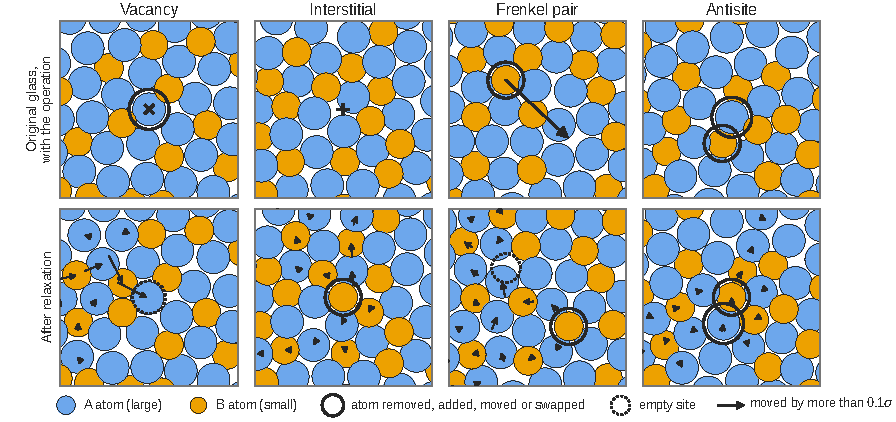
\includegraphics[width=0.72\linewidth]{figures/pd_fig1_defects.pdf}
\caption{\textbf{The four point defects.} Top: a region of the original glass and the operation that makes the defect ($\times$, atom removed; $+$, atom added; arrow, atom moved; two rings, species exchanged). Bottom: the same region after relaxation, which is the input of the finder; arrows show atoms that moved by more than $0.1\sigma$. In the vacancy, neighbours have moved into the empty site.}
\label{fig:defects}
\end{figure}

Each glass holds 256 atoms, 65\% large A and 35\% small B, in a periodic square box of side $14.6\sigma$, and is an energy minimum of the Kob--Andersen potential (Methods). We made 800 training, 100 validation and 100 test glasses. In each we created a defect by a single operation (Fig.~\ref{fig:defects}): removing an atom (vacancy), inserting a B atom at the most open point near a random position (interstitial), moving an atom $1.2$--$3\sigma$ to an open point (Frenkel pair), or exchanging an A atom with its nearest B atom (antisite). The glass was then relaxed again to an energy minimum. Every training glass received eight defects of each type and every validation and test glass two.

Relaxation spreads every defect over many atoms (\supp{tab:physics}). The median number of other atoms that move by more than $0.1\sigma$ ranges from \pd{ph-moved-min} for vacancies to \pd{ph-moved-max} for Frenkel pairs. \pd{vacancy-open}\% of the vacancies remain more open than 95\% of the sites in defect-free glass; in the rest, neighbours have moved into the hole, as found in Lennard-Jones glasses\citep{bennett1979,delaye1993}. The inserted B atom ends with a nearest-neighbour distance of $\pd{ph-int-nn}\sigma$ and an energy of $\pd{ph-int-e}\epsilon$ (medians), close to the $\pd{ph-int-nn-free}\sigma$ and $\pd{ph-int-e-free}\epsilon$ of a B atom in defect-free glass, so it looks much like an ordinary B atom. Frenkel pairs and antisites raise the energy of the glass in \pd{ph-fp-above}\% and \pd{ph-as-above}\% of cases (medians $\pd{ph-fp-e}\epsilon$ and $\pd{ph-as-e}\epsilon$).

A quarter of the Frenkel pairs undid themselves on relaxation: the moved atom pushed a neighbour of its own species into the empty site, and the relaxed glass equals the original up to the exchange of two identical atoms. We excluded these \pd{occ-undone-n} from the test, which leaves \pd{n-test} test defects (\pd{n-vacancy} vacancies, \pd{n-interstitial} interstitials, \pd{n-antisite} antisites and \pd{n-frenkel} Frenkel pairs). To see what the other relaxed defects contain, we assigned every atom of the relaxed glass to the nearest site of the original glass (Methods). This site-occupancy rule recovers \pd{occ-vac}\% of the test vacancies and \pd{occ-int}\% of the interstitials, and classifies all \pd{occ-undone-n} undone Frenkel pairs as defect-free. But only \pd{fp-n-pair} of the \pd{n-frenkel} test Frenkel pairs are still an empty site and a doubly occupied site more than one neighbour shell apart (\supp{tab:occupancy}). The others relaxed into close pairs (\pd{fp-n-close}), antisite-like exchanges (\pd{fp-n-anti}), more complex arrangements (\pd{fp-n-complex}) or no defect (\pd{fp-n-none}). A Frenkel pair is therefore well defined by the operation that made it, but often not by the structure that results.

\subsection*{The finder and how it is scored}

\begin{figure}[t]
\centering
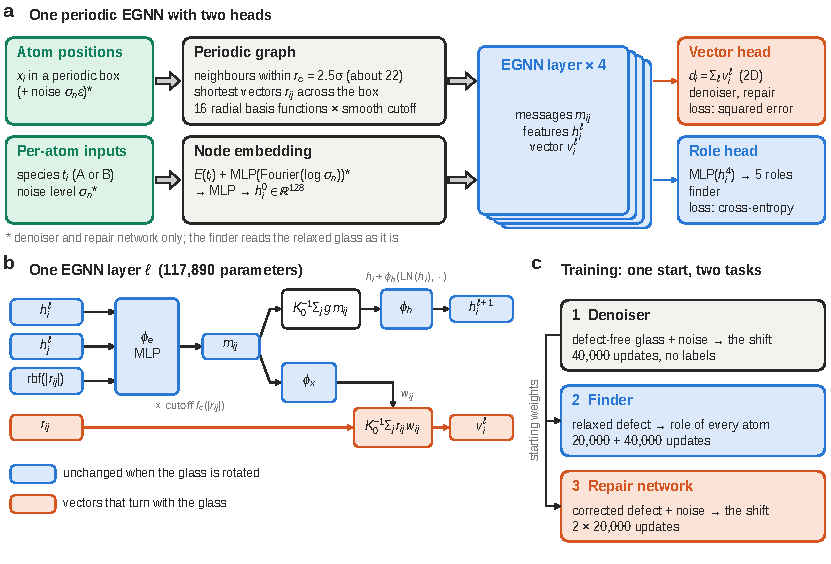
\includegraphics[width=0.9\linewidth]{figures/pd_fig4_network.pdf}
\caption{\textbf{The network.} \textbf{a} The positions define a periodic graph, and the species (and, for the denoiser, the noise level) give the starting features. Four EGNN layers turn both into 128 features and a vector for every atom. The vector head gives the denoiser and the repair network, the role head the finder. \textbf{b} One EGNN layer. Blue quantities do not change when the glass is rotated, orange ones rotate with it. \textbf{c} Training order: the denoiser first, without labels; its weights start the finder and the repair network.}
\label{fig:network}
\end{figure}

The finder (Fig.~\ref{fig:network}) is a periodic EGNN with four message-passing layers of 128 features and a cutoff of $2.5\sigma$ (Methods; Supplementary Tables~\ref{S-tab:models} and~\ref{S-tab:shapes}). Its features depend only on interatomic distances and species, so its output does not change when the glass is shifted, rotated or its atoms renumbered. It is first trained as a denoiser on defect-free glasses, as in DM2\citep{yang2026dm2}: random Gaussian displacements are added to the atoms and the network predicts them. At a noise level of $0.05\sigma$ the predicted correction points along the true force of the potential, with an average cosine of 0.81, although the network never sees a force. The denoiser's weights then initialise the finder, which assigns every atom one of five roles: intact, next to an empty site, extra atom, displaced atom, or wrong species. The roles are known from the operation that made the defect. For a defect of known type, the finder flags the atom with the highest probability for the matching role.

We score a defect as \emph{found} when the flagged atom lies within $1.5\sigma$ of the defect site, about one neighbour shell (for a Frenkel pair or an antisite, of either of its two sites). A randomly chosen atom meets this test in \pd{chance-min}--\pd{chance-max}\% of cases. We score a glass as \emph{restored} when correcting the atoms at the flagged site and minimising the energy returns the original glass, that is, the same inherent structure\citep{stillinger1982}. The correction depends on the defect type, which is taken as known: an atom of the missing species is added at the most open point near a flagged vacancy, a flagged interstitial is removed, a flagged displaced atom is moved to a nearby open point, and a neighbouring A--B pair is exchanged for an antisite (Methods; \suppfig{fig:pipeline}).

\subsection*{The finder locates more defects than classical measures}

% copy of fr_table_results.tex written by make_manuscript_tables.py
% written by make_final_numbers.py
\begin{table}[t]
\centering
\caption{\textbf{Finding and restoring the test defects.} Shares in \%. Found: the flagged atom lies within $1.5\sigma$ of the defect (for a Frenkel pair, of either end; the finder flags the displaced atom itself in \pd{frenkel-exact-finder}\%, the atom energy in \pd{frenkel-exact-energy}\%). Restored: the original glass is recovered after correcting the atoms at the flagged atom and minimising the energy. Brackets: 95\% intervals. Bold: the best method. Only the atom energy uses the potential to flag the atom; every repair ends with minimisation.}
\label{tab:found}\label{tab:restored}
\footnotesize\setlength{\tabcolsep}{3pt}
\begin{tabular}{@{}lcccccc@{}}
\toprule
Defect & $n$ & Learned finder & Cell size & Unlike neighb. & Atom energy & Reference \\
\midrule
\multicolumn{6}{@{}l}{\emph{Found}} & \emph{random atom} \\
Vacancy & 200 & \textbf{69.5} {\scriptsize[62, 76]} & 47.5 {\scriptsize[40, 55]} & 29 {\scriptsize[22, 36]} & 29.5 {\scriptsize[23, 36]} & 2.9 \\
Interstitial & 200 & \textbf{50} {\scriptsize[42, 57]} & 15 {\scriptsize[10, 20]} & 28 {\scriptsize[22, 34]} & 28 {\scriptsize[22, 34]} & 3 \\
Antisite & 200 & \textbf{49} {\scriptsize[42, 56]} & 16.5 {\scriptsize[12, 22]} & 31.5 {\scriptsize[25, 38]} & 29 {\scriptsize[23, 35]} & 4 \\
Frenkel pair & 150 & \textbf{45.3} {\scriptsize[38, 53]} & 26.7 {\scriptsize[20, 33]} & 27.3 {\scriptsize[21, 34]} & 32.7 {\scriptsize[25, 40]} & 5.4 \\
\addlinespace
\multicolumn{6}{@{}l}{\emph{Restored}} & \emph{true location given} \\
Vacancy &  & \textbf{53.5} {\scriptsize[46, 61]} & 40.5 {\scriptsize[34, 48]} & 22 {\scriptsize[16, 28]} & 26 {\scriptsize[20, 32]} & 67 {\scriptsize[60, 74]} \\
Interstitial &  & \textbf{38} {\scriptsize[31, 46]} & 8.5 {\scriptsize[4, 13]} & 21.5 {\scriptsize[16, 27]} & 21 {\scriptsize[16, 26]} & 80 {\scriptsize[74, 86]} \\
Antisite &  & \textbf{30} {\scriptsize[24, 36]} & 1.5 {\scriptsize[0, 4]} & 7.5 {\scriptsize[4, 11]} & 8 {\scriptsize[4, 12]} & 68.5 {\scriptsize[62, 74]} \\
Frenkel pair &  & \textbf{12.7} {\scriptsize[8, 18]} & 0 {\scriptsize[0, 2]} & 1.3 {\scriptsize[0, 3]} & 7.3 {\scriptsize[3, 11]} & 42 {\scriptsize[34, 50]} \\
\bottomrule
\end{tabular}
\end{table}


We compared the finder with four classical measures. Each flags one atom per defect, which then goes through the same correction and minimisation (Methods; \suppfig{fig:baselines}): the area of the atom's Voronoi cell (cell size), the number of nearest neighbours of the other species (unlike neighbours), the atom's share of the potential energy (atom energy) and its local pressure. The first two use only positions and species, like the finder; the last two need the potential. For each measure and defect type, the rule (largest, smallest or most unusual value relative to the usual value for the species) was chosen on the validation glasses.

The finder locates \pd{found-finder-vacancy}\% of vacancies, \pd{found-finder-interstitial}\% of interstitials, \pd{found-finder-antisite}\% of antisites and \pd{found-finder-frenkel}\% of Frenkel pairs (Table~\ref{tab:found}; \suppfig{fig:results}). For the first three types this is \pd{lead-found-min}--\pd{lead-found-max} percentage points more than the best classical measure, and the lead over each measure is significant (paired McNemar test, $\pd{p-worst-found}$ after Holm's correction for \pd{n-tests-family} comparisons; \supp{tab:pvalues}). For Frenkel pairs the finder leads the atom energy by \pd{lead-found-frenkel} points (\pd{found-finder-frenkel}\% against \pd{found-energy-frenkel}\%, $p=\pd{p-found-energy-frenkel}$). Local pressure, the probe used for interstitials in the earliest study of this kind\citep{laakkonen1988}, finds \pd{press-min}--\pd{press-max}\% of the defects, fewer than unlike neighbours and atom energy for every type (\supp{tab:species}).

Each classical measure sees one side of a defect. Cell size is competitive only for vacancies (\pd{found-geometry-vacancy}\%), where missing volume is what it looks for, and finds few interstitials and antisites (\pd{found-geometry-interstitial}\% and \pd{found-geometry-antisite}\%). Unlike neighbours and atom energy find similar shares of every type (\pd{found-bonds-min}--\pd{found-energy-max}\%). In defect-free glass the energy of an atom follows its number of unlike neighbours closely (correlation $-0.90$ for A atoms and $-0.84$ for B atoms), because the A--B attraction is by far the strongest in this mixture\citep{kob1995}. For locating defects, the potential therefore adds little to a count of neighbours.

The largest difference appears for vacancies of small atoms. The atom energy finds \pd{vacA-found-energy}\% of the vacancies left by A atoms but only \pd{vacB-found-energy}\% of those left by B atoms, and cell size finds \pd{vacA-found-geometry}\% and \pd{vacB-found-geometry}\%. The finder locates both alike (\pd{vacA-found-finder}\% and \pd{vacB-found-finder}\%; \supp{tab:species}). A missing B atom leaves little trace on any single neighbour, but the finder reads the change over several of them. For the Frenkel pairs that remain true pairs after relaxation (\pd{fpair-n} of \pd{n-frenkel}), the finder finds \pd{fpair-found-finder}\% and the atom energy \pd{fpair-found-energy}\% (\pd{fpair-p-found-energy}); on this small subset the difference is not significant.

\subsection*{Restoring the glass}

With the finder's flag, correction and minimisation restore \pd{restored-finder-vacancy}\% of the vacancy glasses, \pd{restored-finder-interstitial}\% of the interstitial glasses, \pd{restored-finder-antisite}\% of the antisite glasses and \pd{restored-finder-frenkel}\% of the Frenkel-pair glasses (Table~\ref{tab:restored}). This is more than with any classical measure ($\pd{p-worst-restored}$ against each measure for the first three types; for Frenkel pairs \pd{restored-finder-frenkel}\% against \pd{restored-energy-frenkel}\%, $p=\pd{p-restored-energy-frenkel}$). Given the true location, the same procedure restores \pd{restored-ceiling-min}--\pd{restored-ceiling-max}\%. For vacancies, interstitials and antisites, finding the defect, not repairing it, therefore limits the result. Frenkel pairs are hard to restore even from the true location (\pd{restored-ceiling-frenkel}\%), in line with the rearrangements found by the site-occupancy analysis.

Can a network replace the minimisation? We fine-tuned the denoiser into a repair network that predicts, for each atom of the corrected glass, the displacement back to the original (Methods). It moves the displaced atoms in the right direction: one step removes \pd{repair-removed-v2}\% of their distance from the original positions. But when minimisation follows, applying the repair network first changes the restored rates by less than their statistical uncertainty. Used on its own it pushes atoms onto each other: after one step, \pd{repair-overlap-1}\% of the glasses (depending on the defect type) contain two atoms closer than any pair in the data, and after ten steps \pd{repair-overlap-10}\%. A network trained only on distances to a target has no notion that atoms cannot overlap; the potential supplies it.

\subsection*{What the finder needs}

% written by make_manuscript_tables.py
\begin{table}[t]
\centering
\caption{\textbf{Effect of design choices.} Share of the test defects found (\%), calibrated. Each row is the mean over training runs that differ only in the random seed (Runs); the spread between runs (standard deviation) follows the $\pm$. Start: initial weights, from the denoiser or random. The two lower EGNN rows from the denoiser are single runs. Short ablation runs are scored with their final weights, the 20,000-update runs with the moving average of the weights.}
\label{tab:design}
\footnotesize\setlength{\tabcolsep}{3.5pt}
\begin{tabular}{@{}lllcccccl@{}}
\toprule
Finder & Start & Updates & Runs & Vacancy & Interst. & Antisite & Frenkel & All \\
\midrule
\multicolumn{9}{@{}l}{\emph{Ablations of the EGNN finder (2,000 updates)}} \\
Reference: 4 layers, class weights & denoiser & 2,000 & 3 & 63.0 & 30.7 & 41.7 & 38.7 & 43.8 $\pm$ 0.8 \\
Random initialisation & random & 2,000 & 3 & 14.3 & 26.8 & 24.2 & 22.2 & 21.9 $\pm$ 2.8 \\
Random initialisation, 2 layers & random & 2,000 & 3 & 13.8 & 26.5 & 20.8 & 21.3 & 20.6 $\pm$ 2.4 \\
Random initialisation, 1 layer & random & 2,000 & 3 & 12.3 & 21.8 & 14.2 & 13.8 & 15.6 $\pm$ 1.5 \\
No class weights & denoiser & 2,000 & 3 & 63.2 & 31.0 & 39.5 & 35.1 & 42.7 $\pm$ 1.0 \\
Without self-annihilated Frenkel pairs & denoiser & 2,000 & 3 & 64.7 & 30.8 & 40.2 & 38.0 & 43.8 $\pm$ 2.1 \\
\addlinespace
\multicolumn{9}{@{}l}{\emph{Kind of network}} \\
Transformer & random & 20,000 & 3 & 67.2 & 48.3 & 54.2 & 42.0 & 53.6 $\pm$ 0.3 \\
CNN (U-Net) & random & 20,000 & 3 & 69.7 & 51.2 & 52.8 & 38.4 & 54.0 $\pm$ 0.5 \\
EGNN & random & 20,000 & 3 & 63.2 & 29.7 & 44.0 & 35.1 & 43.5 $\pm$ 0.5 \\
EGNN & denoiser & 20,000 & 1 & 67.0 & 47.5 & 46.5 & 36.7 & 50.3 \\
EGNN (finder of Table 1) & denoiser & 60,000 & 1 & 69.5 & 50.0 & 49.0 & 45.3 & 54.0 \\
\bottomrule
\end{tabular}
\end{table}


To see which parts of the method matter, we trained short finders (\pd{abl-updates} updates) in six settings, with three random seeds each (Table~\ref{tab:design}). Starting from the denoiser doubles the share of defects found, \pd{abl-reference-all}\% against \pd{abl-scratch-all}\% from random weights, and the denoiser start is ahead in every seed. The gain is largest for vacancies (\pd{abl-reference-vacancy}\% against \pd{abl-scratch-vacancy}\%), which matches what the denoiser already knows: ranking the atoms by the size of its predicted correction, before any training on defects, finds 44\% of the test vacancies but few interstitials and antisites. From random weights, one layer finds fewer defects than four (\pd{abl-layers1-all}\% against \pd{abl-scratch-all}\%). Removing the class weights from the loss, or the undone Frenkel pairs from training, changes the result by about one point or less, within the spread between seeds.

With longer training the benefit of the denoiser start shrinks. After 20,000 updates the finder started from the denoiser finds \pd{fin-pre-all}\% of the test defects and the EGNN from random weights \pd{fin-egnn-all}\% (mean of three seeds). The main finder was trained for 60,000 updates, the last 40,000 at half the learning rate, which raised the share found from \pd{exp-20k}\% to \pd{exp-60k}\% (\pd{exp-p-length}). It does not overfit: it finds \pd{split-train-all}\% of the training defects, \pd{split-val-all}\% of the validation defects and \pd{split-test-all}\% of the test defects, with similar loss on all three (\supp{tab:splits}; \suppfig{fig:training}).

\subsection*{Graph, attention or convolution}

\begin{figure}[t]
\centering
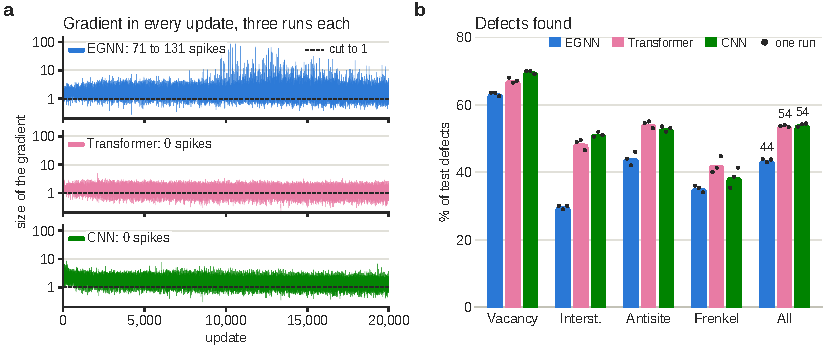
\includegraphics[width=0.92\linewidth]{figures/pd_fig5_finders.pdf}
\caption{\textbf{Three kinds of network trained alike from random weights.} \textbf{a} Gradient norm at every update, before clipping to 1 (dashed line), for three runs of each network; logarithmic axis. \textbf{b} Test defects found, by defect type. Bars are means of three runs, dots single runs.}
\label{fig:finders}
\end{figure}

The EGNN is one of several reasonable choices. We also trained a transformer, in which every atom attends to every other with a learned bias from their distance across the periodic box\citep{ying2021graphormer}, and a CNN, a U-Net\citep{ronneberger2015unet} applied to the glass drawn as a two-channel image with periodic padding (Methods). Both have about half a million parameters, like the EGNN, and were trained in the same way as an EGNN from random weights, with three seeds for 20,000 updates each (Fig.~\ref{fig:finders}, Table~\ref{tab:design}). The transformer finds \pd{fin-tr-all}\% and the CNN \pd{fin-cnn-all}\% of the test defects, against \pd{fin-egnn-all}\% for the EGNN. Each is ahead of the EGNN in every seed (\pd{fin-p-tr}), and the two do not differ from each other (McNemar \pd{fin-p-tr-cnn} across the three seeds). The gain is mostly in interstitials and antisites. Without pre-training and with a third of the updates, both match the main finder (\pd{fin-main-all}\%).

Every training run recorded the gradient norm at every update (Fig.~\ref{fig:finders}a; \supp{tab:stability}). The EGNN shows \pd{stab-egnn-gspikes} gradient spikes per 20,000-update run (a gradient more than five times the median of the previous 100 updates), with gradient norms up to \pd{stab-egnn-largest}; the transformer and the CNN show none, with largest norms of \pd{stab-tr-largest} and \pd{stab-cnn-largest}. With the gradient norm clipped at 1, no run diverged, and the three runs of each 20,000-update recipe agree within one percentage point.

The three networks largely fail on the same defects. With the same seed, \pd{fin-by-none}\% of the test defects are found by none of them, and averaging the outputs of all six transformer and CNN runs finds \pd{fin-six-all}\%, not significantly more than the best single run (\pd{fin-six-p}).

\subsection*{What the finder has learned, and how it fails}

\begin{figure}[t]
\centering
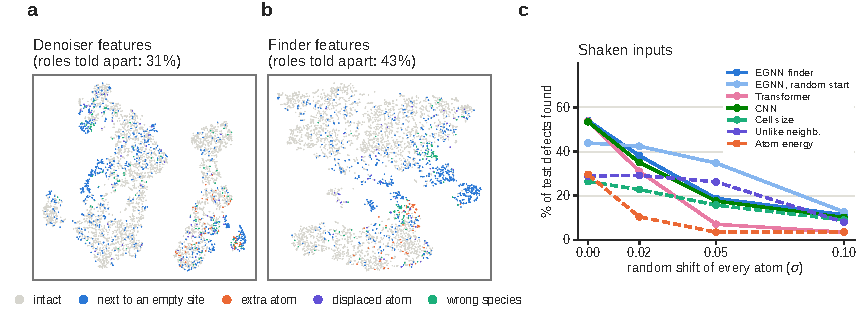
\includegraphics[width=\linewidth]{figures/fr_fig_features.pdf}
\caption{\textbf{Learned features and sensitivity to displacements.} \textbf{a},\textbf{b} The 128 features after the last layer for \pd{feat-atoms} atoms of the test glasses (every atom with a defect role and a sample of intact ones), embedded in two dimensions with t-SNE and coloured by true role: \textbf{a} the denoiser, before any defect labels; \textbf{b} the finder. The two large groups are the two species. In brackets: balanced accuracy of a 5-nearest-neighbour vote on the roles in the full 128 dimensions. \textbf{c} Test defects found when every atom is displaced at random by a Gaussian of the given standard deviation.}
\label{fig:features}
\end{figure}

Fig.~\ref{fig:features}a,b shows the features of the atoms after the last layer, embedded in two dimensions with t-SNE\citep{maaten2008}. In both the denoiser and the finder the two large groups are the two species. In the denoiser's map the atoms with defect roles are scattered among intact atoms. In the finder's map part of the atoms next to an empty site form their own group, and extra and wrong-species atoms gather together, but many defect atoms still lie among intact ones. A vote of the five nearest neighbours in the full 128-dimensional space separates the five roles with a balanced accuracy of \pd{knn-den}\% for the denoiser and \pd{knn-fin}\% for the finder (chance 20\%). Training on defects sharpens the features, but only in part.

The EGNN and the transformer flag the same atom when the glass is shifted, rotated by $90^\circ$ or its atoms renumbered, for every test defect, as their construction guarantees. The CNN changes its flag after a random shift for \pd{fin-cnn-noshift}\% of the defects, because an image has a pixel grid. Random displacements are a harder test (Fig.~\ref{fig:features}c). Displacing every atom by a Gaussian of standard deviation $0.02\sigma$ lowers the main finder from \pd{noise-fin-0}\% to \pd{noise-fin-20}\%, the transformer from \pd{noise-tr-0}\% to \pd{noise-tr-20}\% and the CNN from \pd{noise-cnn-0}\% to \pd{noise-cnn-20}\%. The atom energy falls from \pd{noise-energy-0}\% to \pd{noise-energy-20}\%, because the energy rises steeply when two atoms approach. The count of unlike neighbours does not change (\pd{noise-bonds-20}\%), and the EGNN trained from random weights, the weakest finder, loses little (\pd{noise-scr-20}\%). At $0.1\sigma$ no method finds more than \pd{noise-max-last}\%. Trained only on fully relaxed glasses, the stronger networks rely on fine detail of the relaxed structure that small displacements destroy.

Finally, the finder says where a defect is, not whether there is one. On a mix of defect-free and defected test glasses, its highest role probability separates the two with an area under the ROC curve of only \pd{glass-auc}.

\section*{Discussion}

Because the four standard point defects can be created by simple operations and relaxed with the true potential, the right answer is known exactly. On this benchmark a network that reads only positions and species locates relaxed vacancies, interstitials and antisites \pd{lead-found-min}--\pd{lead-found-max} points more often than the best of four classical measures, two of which use the potential. The advantage is largest where single-atom measures fail by construction. A missing small atom leaves no single neighbour with a large cell or a high energy. An interstitial that has made room for itself looks like an ordinary B atom. An antisite is a fault of chemical order that cell size cannot see. The finder reads changes spread over several atoms and, as the vacancies of B atoms show, does not share the species-dependent blind spots of the classical measures.

Once a defect is located, the physics does the rest. Correcting the number or species of atoms at the flagged site and minimising the energy restores the glass, while a learned repair network adds nothing when minimisation follows and breaks physical realism when used alone. These results suggest a division of labour: the network locates, and the potential, where it is known, repairs. Where no potential is available, the repair step remains open.

Three results concern the choice of method. Denoising pre-training speeds up learning, doubling what the finder learns in 2,000 updates, but its benefit shrinks with longer training. The kind of network matters more: a transformer and a CNN trained from random weights find ten points more than the EGNN trained like them, and match the pre-trained EGNN with a third of its training. We have not identified the cause. The EGNN also showed gradient spikes that the other two did not, but clipping kept every run stable and repeatable. Finally, all three networks miss about the same third of the defects, so a different network alone is unlikely to close the gap; the missed defects may need a different input or a different definition of success.

The study has clear limits. (i) The defects are put in by hand. They are controlled test cases with a known answer, not a model of how defects form in real glasses, where atoms often move collectively\citep{faupel2003}. (ii) The finder needs no potential once trained, but its training data come from one. (iii) The glass is two-dimensional, has 256 atoms and is at zero temperature; each glass holds one defect of known type, and the interstitial is always a B atom. (iv) The main finder was trained once; its intervals cover the variation of the test sample, not of training. The ablations and the comparison of networks use three seeds each. Some development choices (the length of training, the second version of the repair network and the exclusion of undone Frenkel pairs) were made after results of an earlier version on the test defects had been seen. (v) Small random displacements remove most of the networks' lead. Applied to thermally vibrating or measured structures, a finder trained on relaxed glasses could report confident but wrong defects.

The next steps follow from these limits: training on displaced inputs so that the finder tolerates vibration and measurement error; predicting the type of defect and whether a glass has one, with labels from site occupancy; and moving to three-dimensional network glasses such as silica, where both relaxation and identification are harder.

\section*{Methods}

\subsection*{Glasses}
We used the two-dimensional Kob--Andersen mixture\citep{kob1995,bruning2009} with 65\% A and 35\% B atoms and the pair potential
\begin{equation}
U=\sum_{i<j}\phi_{t_it_j}(r_{ij}),\qquad \phi_{ab}(r)=4\epsilon_{ab}\Big[\big(\tfrac{\sigma_{ab}}{r}\big)^{12}-\big(\tfrac{\sigma_{ab}}{r}\big)^{6}\Big],
\label{eq:potential}
\end{equation}
cut and shifted at $2.5\sigma_{ab}$, with $\epsilon_{AA}=1$, $\epsilon_{AB}=1.5$, $\epsilon_{BB}=0.5$, $\sigma_{AA}=1$, $\sigma_{AB}=0.8$ and $\sigma_{BB}=0.88$. Here $r_{ij}$ is the distance between atoms $i$ and $j$ across the periodic box and $t_i\in\{A,B\}$ the species; lengths are in units of $\sigma=\sigma_{AA}$ and energies in units of $\epsilon=\epsilon_{AA}$. With LAMMPS\citep{thompson2022lammps} we melted $N=256$ atoms in a square periodic box of side $L=14.6\sigma$ (number density 1.20) at temperature $T=2$, cooled them at a rate of $10^{-2}$ per unit of time to $T=0.01$, and minimised the energy. This gave 800 training, 100 validation and 100 test glasses. Every glass was relaxed with the FIRE minimiser\citep{bitzek2006fire} until the largest force was below $10^{-8}$, and no two atoms were closer than $0.56\sigma$.

\subsection*{Defects and labels}
Each defect was made by one operation on a defect-free glass, followed by FIRE relaxation in a fixed box to the same force tolerance. A \emph{vacancy} removes one atom of either species (255 atoms). An \emph{interstitial} adds a B atom at the most open point within $2\sigma$ of a random position (257 atoms). A \emph{Frenkel pair} moves one atom to the most open point $1.2$--$3\sigma$ from its site. An \emph{antisite} exchanges the species of an A atom and its nearest B atom. The most open point is the point of a grid of spacing $0.05\sigma$ farthest from every atom within the stated range. Each training glass received 8 defects of each type (6,400 per type) and each validation and test glass 2 (200 per type). A Frenkel pair whose relaxed glass is the original glass again, by the test used for restoring below (which allows identical atoms to exchange places), was counted as undone; the 50 undone test pairs were excluded from the test.

Every atom of a defected glass has one of five roles $y_i$, known from the operation: intact; next to an empty site (first-shell neighbours of the removed atom, or of the original site of a moved atom, within $1.4\sigma_{t_it_j}$); extra atom; displaced atom; wrong species (both exchanged atoms). Over 98\% of the atoms are intact.

\subsection*{Site-occupancy analysis}
To judge what a relaxed defect contains, every atom of the relaxed glass was assigned to the nearest site of the original glass, as one compares a crystal with its lattice. A site can then be empty, singly or doubly occupied. A relaxed defect was classed as a vacancy if one site was empty and none doubly occupied, as an interstitial if one site was doubly occupied and none empty, as a Frenkel pair if one site was empty and one doubly occupied more than one neighbour shell ($1.4\sigma_{\alpha\beta}$ for the species of the two sites) apart, and as a close pair if they were closer. If every site held one atom, the defect was classed as antisite-like when some sites held an atom of the other species and as no defect otherwise; all other cases were classed as complex (\supp{tab:occupancy}).

\subsection*{Classical measures}
Nearest neighbours are atoms closer than $1.4\sigma_{t_it_j}$. \emph{Cell size} is the area of the atom's Voronoi cell\citep{starr2002}; \emph{unlike neighbours} is the number of nearest neighbours of the other species; \emph{atom energy} is $\tfrac12\sum_j\phi_{t_it_j}(r_{ij})$; \emph{local pressure} is $w_i=\tfrac12\sum_j\big(-r_{ij}\,\mathrm{d}\phi_{t_it_j}/\mathrm{d}r_{ij}\big)$ divided by twice the mean area per atom. The per-atom virials $w_i$ sum to the pressure of the box times twice its area, which we checked against the change of energy under a small change of the box. Each value is compared with the mean and spread for the species in defect-free glass. On the validation glasses we chose, for each measure and defect type, whether to flag the largest, the smallest or the most unusual value; atoms with equal values were ranked at random. Forces cannot be used, because they vanish in a relaxed glass.

\subsection*{EGNN}
Atoms closer than $r_c=2.5\sigma$ are connected; $r_{ij}$ is the shortest vector between them across the box, expanded in 16 Gaussian radial functions (rbf) with a smooth cutoff $f_c$. Starting from an embedding of the species, $h_i^0=\mathrm{MLP}(E(t_i))\in\mathbb R^{128}$ with $E$ a learned table (the denoiser adds 64 random Fourier features of $\log\sigma_n$), each of four layers computes
\begin{equation}
\begin{aligned}
m_{ij}&=\phi_e\big(h_i,h_j,\mathrm{rbf}(|r_{ij}|)\big)f_c(|r_{ij}|),\qquad
h_i\leftarrow h_i+\phi_h\Big(\mathrm{LN}(h_i),\tfrac{1}{K_0}\textstyle\sum_j g(m_{ij})m_{ij}\Big),\\
v_i^\ell&=\tfrac{1}{K_0}\textstyle\sum_j r_{ij}\,\phi_x(m_{ij})f_c(|r_{ij}|),
\end{aligned}
\label{eq:layer}
\end{equation}
with two-layer networks $\phi_e,\phi_h,\phi_x$ (SiLU activation), a sigmoid gate $g$, layer normalisation LN and $K_0=24$. The features $h_i$ depend only on distances and species, so they are invariant to shifts, rotations and renumbering. The vector $d_i=\sum_\ell v_i^\ell$ rotates with the glass and has the form of a force; it is the output of the denoiser and the repair network. The finder's role head is $P_i=\operatorname{softmax}\big(W_2\,\mathrm{SiLU}(W_1h_i^4)\big)$ with $W_1\in\mathbb R^{128\times128}$ and $W_2\in\mathbb R^{5\times128}$. Four layers reach $10\sigma$, more than half the box. The finder has \pd{size-egnn} parameters and the denoiser \pd{size-den}; Supplementary Table~\ref{S-tab:shapes} lists every block.

\subsection*{Transformer and CNN}
In the transformer, each atom starts from its species and its surroundings, $h_i^0=E(t_i)+\mathrm{MLP}(\rho_i)$, where $\rho_i\in\mathbb R^{2\times16}$ counts the neighbours of each species within $2.5\sigma$ in 16 Gaussian distance bins. Every pair of atoms gets features $e_{ij}=\mathrm{MLP}(\mathrm{rbf}_{32}(|r_{ij}|))\in\mathbb R^{64}$ from its distance across the box. Each of four pre-norm blocks computes, for 8 heads $k$ of 16 dimensions,
\begin{equation}
a^{k}_{ij}=\operatorname{softmax}_j\Big(\tfrac{1}{4}\,q_i^{k}\cdot \kappa_j^{k}+w_k^\top e_{ij}+c_k\Big),\quad
h_i\leftarrow h_i+W_o\big[\textstyle\sum_j a^k_{ij}u_j^k\big]_{k=1}^{8},\quad
h_i\leftarrow h_i+\mathrm{FFN}(\mathrm{LN}(h_i)),
\label{eq:attention}
\end{equation}
where the queries, keys and values $q,\kappa,u$ are linear maps of $\mathrm{LN}(h)$ and the feed-forward network FFN has 256 hidden units. The distance term $w_k^\top e_{ij}+c_k$ lets each head attend near or far. Only distances enter, so the output is invariant to shifts, rotations and renumbering. The role head is as for the EGNN (\pd{size-tr} parameters).

For the CNN, the glass is drawn as a two-channel image, $I_s(p)=\sum_{i:\,t_i=s}\exp\big(-\lVert p-x_i\rVert_L^2/2b^2\big)$ for species $s$, on a $128\times128$ grid of pixel centres $p$ ($0.11\sigma$ per pixel, $b=0.15\sigma$), so that positions finer than a pixel still show. A U-Net with five levels (16 to 96 channels; at each level two $3\times3$ convolutions with group normalisation and SiLU; $2\times2$ average pooling on the way down, nearest-neighbour upsampling and skip connections on the way up) returns 16 features per pixel. Convolutions pad circularly, so the image wraps around like the box. The features at each atom are read by bilinear interpolation, joined to a species embedding and passed through a head $32\to64\to5$ (\pd{size-cnn} parameters in total). Training applies one of the 8 rotations by $90^\circ$ and reflections of the square box and a random shift to each glass; testing averages the outputs over all 8.

\subsection*{Training}
\emph{Denoiser.} A defect-free glass $X_0$ is displaced by noise of size $\sigma_n\sim\mathcal U(0.001,1)$, $X=X_0+\sigma_n\varepsilon$ with $\varepsilon\sim\mathcal N(0,I)$, and the network predicts the displacement:
\begin{equation}
\mathcal L_{\text{den}}(\theta)=\mathbb E_{X_0,\sigma_n,\varepsilon}\,\tfrac{1}{N}\textstyle\sum_i\big\lVert d_\theta(X,\sigma_n)_i-(x_i-x_{0,i})\big\rVert^2 .
\label{eq:den}
\end{equation}
Its minimiser is $d^*=-\sigma_n^2\nabla_X\log p_{\sigma_n}(X)$\citep{vincent2011,efron2011}. In thermal equilibrium $\log p=-U/k_BT+\text{const}$, so $d^*$ points along the force $-\nabla U$. Our glasses are not in equilibrium, so we measured the agreement: at $\sigma_n=0.05$ the average cosine between the predicted correction and the force is 0.81. The denoiser was trained for 40,000 updates.

\emph{Finder.} The finder starts from the denoiser's weights (or from random weights, where stated) and is trained with class-weighted cross-entropy over the atoms of a batch $B$:
\begin{equation}
\mathcal L_{\text{find}}(\theta)=-\frac{\sum_{i\in B} w_{y_i}\log P_\theta(y_i\mid\tilde G)_i}{\sum_{i\in B} w_{y_i}},\qquad w_c=(n_c/n_0)^{-1/2},
\label{eq:find}
\end{equation}
where $\tilde G$ is the defected glass and $n_c$ the number of training atoms with role $c$, which gives weights of 1, 9.2, 31.7, 31.8 and 22.4 for the five roles in the order listed above. Because the weights inflate the rare roles, test outputs are calibrated by logit adjustment\citep{menon2021}, $P_i=\operatorname{softmax}(z_i-\log w)$, with $z_i$ the network's outputs. Each update draws one defect type with probability $1/4$ (a batch holds one type, since the number of atoms differs), makes the batch defect-free with probability 0.2, and draws 16 glasses of that type uniformly with replacement from the training split. The main finder was trained for 20,000 updates and then 40,000 at half the learning rate. Every 1,000 updates the moving-average weights were scored on 200 validation defects of each type. Validation was used to choose the training settings and the rules of the classical measures; the choices made after test results had been seen are listed in the Discussion.

\emph{Optimisation.} All networks use AdamW\citep{loshchilov2019adamw} ($\beta_1=0.9$, $\beta_2=0.999$, $\epsilon=10^{-8}$, weight decay 0) with learning rate $2\times10^{-4}$ (the transformer with a linear warm-up over 1,000 updates), clip the gradient norm at 1, and keep a moving average of the weights with factor 0.999, which is used for testing. A finder update takes 0.2--0.3\,s on one NVIDIA T4 GPU. The models and the settings tried are listed in Supplementary Table~\ref{S-tab:models}.

\emph{Repair network.} The denoiser was fine-tuned to predict, for every atom of the glass with the number and species of atoms corrected at the true defect site, the displacement to its position in the original glass. Small Gaussian noise (log-uniform standard deviation between 0.001 and $0.3\sigma$) was added to the input, and the loss weighted the atoms displaced by the defect 11 times more than the rest.

\subsection*{Correction, repair and success}
For a defect of type $k$ with role $c(k)$, a method flags the atom $\hat\imath=\arg\max_i P_{i,c(k)}$ (for the classical measures, the atom chosen by the rule). With $S$ the defect site or sites,
\begin{equation}
\text{found}=\mathbb 1\Big[\min_{s\in S}\lVert \tilde x_{\hat\imath}-s\rVert_L<1.5\sigma\Big],\qquad
\text{restored}=\mathbb 1\big[\operatorname{relax}(\operatorname{correct}_k(\tilde G,\hat\imath))\equiv G\big],
\label{eq:metrics}
\end{equation}
where $\lVert\cdot\rVert_L$ is the distance across the periodic box. The correction adds an atom of the missing species at the most open point within $1.5\sigma$ of $\hat\imath$ (vacancy), removes $\hat\imath$ (interstitial), moves $\hat\imath$ to one of up to eight open points $1$--$3.2\sigma$ away (Frenkel pair), or exchanges a neighbouring A--B pair near $\hat\imath$ (antisite). Where there is a choice, each method chooses with its own score, and the energy route keeps the option with the lowest energy. The corrected glass is relaxed with a FIRE minimiser written in PyTorch (largest force below $10^{-6}$), the same for every method. $G'\equiv G$ means that every original atom has an atom of its species within $0.05\sigma$, one to one. With the true location given, an atom of the removed species is placed at the most open point within $1\sigma$ of the empty site, the added atom is removed, the displaced atom is moved to the most open point within $1\sigma$ of its original site, or the two exchanged species are swapped back.

\subsection*{Statistics}
Intervals are 95\% intervals from 10,000 bootstrap resamples of the 100 test glasses\citep{efron1993}, resampling glasses because the two defects of a glass are not independent; where a rate is exactly 0\%, the exact binomial interval is given. Methods are compared on the same defects with McNemar's exact test\citep{mcnemar1947}. For the 12 comparisons of the finder with the three structural and energy measures over four defect types, $p$ values are corrected with Holm's method\citep{holm1979}. Results over several training runs are given as the mean and the standard deviation between runs that differ only in the random seed.

\subsection*{Feature and perturbation analyses}
For Fig.~\ref{fig:features}a,b we took the features after the last layer for every atom with a defect role in the test glasses and a random sample of intact atoms, embedded them with t-SNE\citep{maaten2008} (perplexity 40), and scored a 5-nearest-neighbour vote on the roles in the full 128 dimensions, fitted on half of the atoms, by its balanced accuracy on the other half. For the symmetry tests each test glass was rotated by $90^\circ$, shifted by a random vector or had its atoms renumbered, and we checked whether the flagged atom stayed the same. For Fig.~\ref{fig:features}c every atom of the relaxed test glasses was displaced by Gaussian noise of standard deviation 0, 0.02, 0.05 or $0.1\sigma$, without relaxation, and every method was scored against the original defect sites, with the classical measures compared with their statistics in defect-free glass.

\section*{Data availability}
The glasses, the defects, the trained models and every result reported here are available at \url{https://github.com/chilalaabubakar/IDL-PROJECT} (branch \texttt{dabo-point-defects})\citep{glassdefects2026}.

\section*{Code availability}
The code for generating the data, training the networks, evaluating all methods and producing every number, table and figure of this paper is available at the same repository under the MIT license.

\section*{Acknowledgements}
We thank Prof.\ Ismaila Dabo (Materials Science and Engineering, Carnegie Mellon University) for his review of an earlier version of this work, which led to this study. GPU time was provided by Kaggle and Google Colab.

\section*{Author contributions}
N.L.\ generated the glasses, implemented the potential and the relaxation, and checked the physics of the defects. S.C.\ designed the defect operations, the success tests, the classical measures and the statistics. A.C.\ built and trained the networks and ran the experiments. G.U.\ designed the correction and repair procedure. M.S.\ made the figures and drafted the manuscript. B.G.\ supervised the project. All authors discussed the results and reviewed the manuscript.

\section*{Competing interests}
The authors declare no competing interests.

\singlespacing
\bibliographystyle{unsrtnat}
{\small\bibliography{refs}}

\end{document}
